\documentclass[fleqn]{article} 
\usepackage[paperwidth=8.5in,paperheight=11in,margin=.75in,headheight=0.27in,headsep=.1in]{geometry}
\usepackage{amsmath,amsfonts,amssymb,graphicx,mathtools,flexisym}
\usepackage{tikz}
\usepackage{tkz-graph}
\usepackage{xcolor}
\usepackage{fancyhdr}
\usepackage{hyperref}
\usepackage{parskip}
\usepackage{scrextend}
\usepackage{multirow}
\usepackage{algorithm, algpseudocode}
\usepackage[shortlabels]{enumitem}
\usetikzlibrary{automata,arrows,positioning,calc}


\begin{document}

\begin{figure}[h!]
\begin{center}
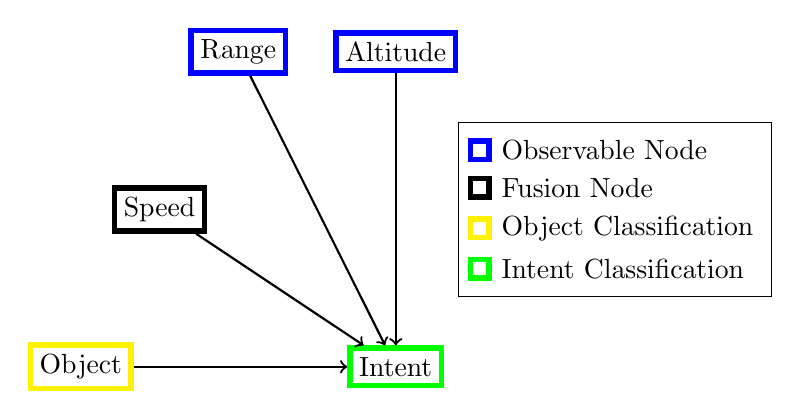
\begin{tikzpicture}[
  bluenode/.style={shape=rectangle, draw=blue, line width=2},
  blacknode/.style={shape=rectangle, draw=black, line width=2},
  yellownode/.style={shape=rectangle, draw=yellow, line width=2},
  greennode/.style={shape=rectangle, draw=green, line width=2}
]
\path
(10,3) node[bluenode, align=center](r1){Range}
(12,3) node[bluenode, align=center](a){Altitude}

(9,1) node[blacknode, align=center](s2){Speed}
(8,-1) node[yellownode, align=center](o){Object}
(12,-1) node[greennode, align=center](i3){Intent};

\draw[->, thick] (r1) -- (i3);
\draw[->, thick] (a) -- (i3);
\draw[->, thick] (s2) -- (i3);
\draw[->, thick] (o) -- (i3);


%Legend creation.
\matrix [draw, right] at (current bounding box.east) {
  \node [bluenode,label=right:Observable Node] {}; \\
  \node [blacknode, label=right:Fusion Node] {}; \\
  \node [yellownode,label=right:Object Classification] {}; \\
  \node [greennode,label=right:Intent Classification] {}; \\
};

\end{tikzpicture}
\end{center}
\caption{\label{fig:1_intent} Intent input nodes and states.}
\end{figure}

\end{document}
